% concatenated from 5_Unlabeled_Chip_Firing_on_Grid.tex
\documentclass[11pt]{article}
\usepackage{amsmath, amssymb, amscd, amsthm, amsfonts, subfig}
\usepackage{graphicx}
\usepackage{verbatim}
\usepackage{float}
\usepackage{color,colortbl}
\usepackage{tikz}
\usepackage{hyperref}

\oddsidemargin 0pt
\evensidemargin 0pt
\marginparwidth 40pt
\marginparsep 10pt
\topmargin -20pt
\headsep 10pt
\textheight 8.7in
\textwidth 6.65in
\linespread{1.2}

\usepackage[font=small,labelfont=bf]{caption}
\usepackage{titlesec}
\expandafter\def\expandafter\normalsize\expandafter{%
    \normalsize%
    \setlength\abovedisplayskip{5pt}%
    \setlength\belowdisplayskip{5pt}%
    \setlength\abovedisplayshortskip{-3pt}%
    \setlength\belowdisplayshortskip{3pt}%
}
\usepackage[scr=boondox, % heavily sloped
            cal=esstix] % slightly sloped
           {mathalpha}
% theorem environment definitions. Change the numbering as needed to fit your paper
\newtheorem{theorem}{Theorem}[section] % reset theorem counter every section

\newtheorem{corollary}[theorem]{Corollary} % reset corollary counter every theorem
\newtheorem{lemma}[theorem]{Lemma} % lemmas, propositions, claims, and conjectures all share numbering with theorems
\newtheorem{proposition}[theorem]{Proposition}
\newtheorem{claim}[theorem]{Claim}
\newtheorem{conjecture}[theorem]{Conjecture}

\theoremstyle{definition}
\newtheorem{definition}{Definition}% definitions, examples, etc. have their numbers
\newtheorem{example}{Example}



\theoremstyle{remark}
\newtheorem*{remark}{Remark} % remarks have no counter. 
\setcounter{secnumdepth}{3}

\newcommand{\floor}[1]{\left\lfloor #1 \right\rfloor}
\newcommand{\ceil}[1]{\left\lceil #1 \right\rceil}

\newcommand\nnfootnote[1]{%
  \begin{NoHyper}
  \renewcommand\thefootnote{}\footnote{#1}%
  \addtocounter{footnote}{-1}%
  \end{NoHyper}
}

%%%%%%%%%%%%%%%%%%%%%%%%%%%%%%%%%%%%%%%%%%%%%%%%%%%%%%%%%%%%%%%%%%%

\DeclareMathOperator{\outdeg}{outdegree}
% Color emph
\newcommand\preceqdot{\mathrel{\ooalign{$\preceq$\cr
  \hidewidth\raise0.225ex\hbox{$\cdot\mkern0.5mu$}\cr}}}





\title{Chip-firing on the Lattice of Nonnegative Integer Points}
\author{Ryota Inagaki \and Tanya Khovanova \and Austin Luo}
\date{}

\begin{document}

\maketitle

\begin{abstract}
Chip-firing on a directed graph is a game in which chips, a discrete commodity, are placed on the vertices of the graph and are transferred between vertices. In this paper, we study a chip-firing game on the Hasse diagram of the lattice of nonnegative integer points on the plane, where we start with $2^n$ chips at the origin. When we fire a vertex $v$, we send one chip to each out-neighbor. We fire until we reach a stable configuration, a distribution of chips where no vertex can fire.

We study the intermediate firing configuration: a table that assigns to each vertex the total number of chips that pass through it. We prove that the nonzero entries of the stable configuration correspond to the odd entries of the intermediate configuration. The intermediate configuration consists of three parts: the top triangle, the midsection, and the bottom triangle. We describe properties of each part. We study properties of each row and the number of rows of the intermediate configuration. We also explore properties of the difference tables, which are tables of first differences of each row of the intermediate firing configuration.
\end{abstract}

\nnfootnote{\emph{2020 Mathematics Subject Classification}:  05A10, 11Y55, 05C57}
\nnfootnote{\emph{Key words and phrases:} Chip-Firing, Pascal's Triangle, Binomial Coefficients} 



\section{Introduction}
Chip-firing is a game on a graph in which a discrete commodity, called chips, is placed on the vertices of the graph. A vertex $v$ fires when it has at least as many chips as neighbors and disperses a chip to each neighbor. In a directed graph, vertices can fire chips only along their out-edges. Chip-firing was initially studied as the Abelian Sandpile, which Bak et al.~\cite{PhysRevLett} and Dhar \cite{dhar1999abelian} explored; in this setting, a stack of sand disperses when it exceeds a certain height. The study of chip-firing on graphs originates from works including Anderson, Lovász, Shor, Spencer, Tardos, and Winograd \cite{zbMATH04135751} and Bj\"orner, Lovász, and Shor \cite{MR1120415}. Since those works were published, numerous variants of chip-firing have been studied, including Biggs’s Dollar Game\footnote{One can play a recreational version of this game at the website \cite{DollarGame}} \cite{MR1676732}, Guzmán and Klivans’s chip-firing game on invertible matrices \cite{MR3311336, MR3504984}, Hopkins, McConville, and Propp’s labeled chip-firing game on 1-dimensional lattices \cite{MR3691530}, Musiker and Nguyen's labeled chip-firing game on undirected binary trees \cite{MR4827886, Inagaki2025}, and the authors' labeled chip-firing on directed trees \cite{MR4887467, inagaki2025permutationbasedstrategieslabeledchipfiring, inagaki2025labeledchipfiringdirectedkary}.

Despite the abundance of work on chip-firing on lattices and trees, relatively little has been written about the chip-firing game on directed graphs that are not trees. Indeed, one aspect that complicates chip-firing games on these graphs is the fact that some chips that diverge from a vertex may reconverge at a different vertex later.

In this paper, we study the chip-firing game on the quadrant lattice graph, which is the Hasse diagram of poset $\mathbb{Z}_{\geq 0}^2$ with coordinate-wise partial order, i.e., $a \leq b$ if the $x$-coordinate of $a$ is less than or equal to that of $b$ and the $y$-coordinate of $a$ is less than or equal to that of $b$. It is one of the simplest and most familiar non-tree posets that come to mind. The quadrant lattice graph is shown in Figure~\ref{fig:quadrantgraph}. 

\begin{figure}[ht!]
    \centering
    \includegraphics[width=0.35\linewidth]{quadrantex.pdf}
    \caption{The quadrant lattice graph with labeled vertices.}
    \label{fig:quadrantgraph}
\end{figure}

We start with $2^n$ chips at the origin $(0, 0)$ and play the chip-firing game until no vertex can fire.

Now we describe the layout of our paper. 

In Section~\ref{sec:prelim}, we introduce preliminary definitions and facts that will be useful in this paper.

Then, in Section~\ref{sec:TotalFirings}, we express the total number of firings required to achieve the stable configuration through the distribution of chips in that configuration.

In Section~\ref{sec:IntermedFiringConfig}, we introduce the intermediate firing configuration, which describes the total number of chips passing through each vertex. We then prove that the nonzero entries of the stable configuration correspond to the odd entries in the intermediate configuration. We present an example where we start with $2^9$ chips and observe interesting structures in the resulting stable configuration.

In Section~\ref{sec:PascalTriangle}, we observe that the first $n+1$ rows of the intermediate configurations are scaled versions of rows of Pascal's Triangle.

In Section~\ref{sec:Med}, we prove that in each row of the intermediate configuration, the entries first strictly increase and later strictly decrease when read from left to right. Then we discuss the number of nonzero entries in each row of the intermediate configuration, which changes by $+1$ or $-1$ when moving to the next row. Afterwards, we give the upper bound on the number of nonzero rows.

In Section~\ref{sec:BottomTriangle}, we discuss the last rows of the intermediate stable configuration, whose nonzero entries form a triangle. These last rows are minimal in some sense and are explicitly described.

Afterwards, in Section~\ref{sec:Discussion}, we summarize our discoveries and show some plots. We also motivate studying the difference tables in the last section. We have extensive computational data that motivates our research. This data can be found in \cite{GithubData}.

Finally, in Section~\ref{sec:DiffTables}, we introduce difference tables, which are differences of consecutive entries in each row of the intermediate configuration, and describe some interesting properties.


\section{Preliminaries}\label{sec:prelim}

\subsection{Unlabeled Chip-Firing}

In the unlabeled chip-firing game on directed graphs, indistinguishable chips are put on the vertices of a directed graph $G = (V, E)$. Vertex $v$ can fire if and only if it has at least $\outdeg(v)$ chips. In other words, vertex $v$ sends one chip to each out-neighbor and consequently loses $\outdeg(v)$ chips.

A \textit{configuration} $\mathcal{C}$ is a distribution of chips over the vertices of a graph. When the firing process reaches a state in which no vertex can fire, the distribution of chips over the vertices is a \textit{stable configuration}.

A key property of unlabeled chip-firing on directed graphs is the following global confluence property, which is analogous to that of chip-firing on undirected graphs (which is similar to Theorem 2.2.2 of Klivans' 
 textbook \cite{klivans2018mathematics}).

\begin{theorem}[Theorem 1.1 of \cite{MR1203679}]\label{thm:confluence}
For a directed graph $G$ and initial configuration $\mathcal{C}$ of chips on the graph, the unlabeled chip-firing game will either run forever or end after the same number of moves and at the same stable configuration. Furthermore, the number of times each vertex fires is the same regardless of the sequence of firings taken in the game.
\end{theorem}



\subsection{Our Setup}

We define the \textit{Hasse diagram of $\mathbb{Z}_{\geq 0}^2$} to be the graph whose vertex set is the set of integer points in the first quadrant, i.e., $\{(x, y): x, y \in \mathbb{Z}_{\geq 0}\}$ and whose edges are $\{(x, y) \to (x+1, y): x, y \in \mathbb{Z}_{\geq 0}\}$ and $\{(x, y) \to (x, y+1): x, y \in \mathbb{Z}_{\geq 0}\}$. We say that a vertex $v = (v_x, v_y)$ is in row $i$ if $v_x+v_y=i$. For vertices  $(a, b)$ and $(c, d)$ that are in the same row, we say that $(a, b)$ is \textit{left} of $(c, d)$ if $b-a < d-c$, or equivalently $b < d$.

Our chip-firing game proceeds on the graph described above. We call the vertex $(0,0)$ \textit{the root}.

In our chip-firing game, we denote the \textit{initial configuration} of chip-firing as placing of $2^n$ chips on the root. A vertex $v=(x, y)$ can \textit{fire} if and only if it has at least $2$ chips. When vertex $v$ \textit{fires}, it transfers a chip from itself to each of its $2$ children.

\begin{example} Figure~\ref{fig:exampleunlabel} shows the unlabeled chip-firing process with $4$ indistinguishable chips initially placed at the origin of the quadrant lattice, where the graph is rotated so edges are directed down.

\begin{figure}[ht!]
\centering
    \subfloat[\centering Initial configuration with $4$ chips]{{\includegraphics[width=0.25\linewidth]{quadunlabeledex1.pdf} }}%
    \qquad
    \subfloat[\centering Configuration after firing once]{{\includegraphics[width=0.25\linewidth]{quadunlabeledex2.pdf} }}%
    \qquad
    \subfloat[\centering Configuration after firing twice]{{\includegraphics[width=0.25\linewidth]{quadunlabeledex3.pdf} }}%
    \qquad
    \subfloat[\centering Configuration after firing four times]{{\includegraphics[width=0.25\linewidth]{quadunlabeledex4.pdf} }}
    \qquad
    \subfloat[\centering Stable configuration]{{\includegraphics[width=0.25\linewidth]{quadunlabeledex5.pdf} }}
    \caption{Example of unlabeled chip-firing on an infinite directed quadrant lattice}%
    \label{fig:exampleunlabel}
\end{figure}
\end{example}

We claim that if we start a chip-firing game with the initial configuration as above, it will always stabilize. Suppose, on the contrary, that we never reach a stable configuration. This means that the number of chips transferred from row $i$ to row $i+1$ must be the same from some row $N$ onward. It means that no chip is left behind, and every vertex on rows $N$ and later receives an even number of chips. Consider the leftmost vertex in row $N$; suppose it receives $a$ chips. Thus, the leftmost vertex in the next row receives $\floor{\frac{a}{2}}$ chips. As this quantity decreases, eventually the leftmost vertex in some row has to receive an odd number of chips. This is a contradiction.

We observe that, as long as we start with the same number of chips at the root, all firing processes lead to the same stable configuration. This is a result of Theorem~\ref{thm:confluence}.


\section{The Total Number of Firings}\label{sec:TotalFirings}

Let us denote by $T(n)$ the total number of firings when we start with $2^n$ chips at the origin. We know that, from the confluence property of chip-firing on directed graphs (Theorem~\ref{thm:confluence}), this number does not depend on the order of firings.

We calculated the first few values of this sequence starting from index 0 (the new sequence A389565 in the OEIS \cite{oeis}):
\[0,\ 1,\ 5,\ 15,\ 52,\ 163,\ 458,\ 1359,\ 4296,\ 12890,\ 38570.\]
% 0, 1, 5, 15, 52, 163, 458, 1359, 4296, 12890, 38570, 120647, 387715, 1201294, 3821513, 11929798, 37988037, 120175359, 379389445, 1207951182, 3828450781.

We would like to introduce the distribution of the number of chips in the stable configuration as a function of $y-x$. In other words, we denote by $D_n(i)$ the number of chips in all the vertices $(x,y)$ in the stable configuration such that $y-x = i$ when we start with $2^n$ chips. We call this distribution \textit{the distance distribution}.

\begin{example}
\label{ex:n=4D}
    We get that the distance distribution $D_4$ is
    \[2,\ 1,\ 2,\ 3,\ 0,\ 3,\ 2,\ 1,\ 2.\] To see this, one can either do direct computation of the stable configuration or consider the table in Example~\ref{ex:n=4}, which is the table for the maximum number of chips at each vertex in the firing process for $n=4$. The odd values in bold correspond to vertices that have one chip in the stable configuration, since each firing removes two chips from the vertex that is fired. One can sum the number of bold vertices in each column to obtain the distance distribution $D_4$.
\end{example}

Note that the distance distribution is symmetric with the middle value zero. Consider the second raw moment $\mu_2'(n)$ of the distribution $D_n(i)$:
\[\mu_2'(n) = \sum_i i^2D_n(i).\]

\begin{proposition}
    We have the following connection:
    \[\mu_2'(n) = 2T(n).\]
\end{proposition}

\begin{proof}
    The second raw moment of the initial distribution is 0. We can consider the second raw moments of the resulting chip distribution after some number of firings. Suppose we have 2 chips at the vertex $(x,y)$. Before firing, they contribute $2(y-x)^2$ to the second moment. After the firing, we have one chip at $(x+1,y)$ and the other at $(x,y+1)$; they contribute
    \[(y-x-1)^2 + (y-x+1)^2 = 2(y-x)^2 + 2.\]
    Thus, each firing increases the second moment by 2. The result follows.
\end{proof}

\begin{example}
    From Example~\ref{ex:n=4D}, we get that
    \[T(4) = \frac{\mu_2'(4)}{2} = \frac{2\cdot 4^2 + 3^2 + 2\cdot 2^2 + 3\cdot 1 + 3\cdot 1 + 2\cdot 2^2+ 3^2 + 2\cdot 4^2}{2}  = 52.\]
\end{example}

Figure~\ref{fig:Distancedistributionfor15} shows the distance distribution for $n=15$.

\begin{figure}[ht!]
    \centering
\begin{tikzpicture}[scale=0.5, x=0.18cm,y=0.015cm]
  % Data: 91 values, indexed k = 0..90 (center at k=45)
  % Axes
  \draw[->] (-0.5,0) -- (90.8,0);
  %node[below] {$k$};
  \draw[->] (0,-30) -- (0,580);
  %node[left] {value};

  % x-axis ticks (every 5 to avoid crowding)
  %\foreach \k in {0,5,...,90} {
    %\draw (\k,0) -- (\k,-12);
    %node[below] {\scriptsize \k};
  %}

  % Optional symmetry axis
  %\draw[dotted] (45,-30) -- (45,580);

  % Points
  \foreach \k/\v in {
    0/545,1/517,2/489,3/461,4/433,5/406,6/380,7/355,8/332,9/310,
    10/290,11/271,12/254,13/253,14/272,15/282,16/292,17/300,18/289,19/309,
    20/312,21/299,22/353,23/358,24/389,25/411,26/425,27/439,28/474,29/495,
    30/514,31/437,32/433,33/427,34/458,35/426,36/423,37/407,38/380,39/360,
    40/321,41/277,42/232,43/186,44/108,45/0,
    46/108,47/186,48/232,49/277,50/321,51/360,52/380,53/407,54/423,55/426,
    56/458,57/427,58/433,59/437,60/514,61/495,62/474,63/439,64/425,65/411,
    66/389,67/358,68/353,69/299,70/312,71/309,72/289,73/300,74/292,75/282,
    76/272,77/253,78/254,79/271,80/290,81/310,82/332,83/355,84/380,85/406,
    86/433,87/461,88/489,89/517,90/545
  }{
    \fill (\k,\v) circle (1.4pt);
  }

  % Polyline
  \draw
    (0,545)--(1,517)--(2,489)--(3,461)--(4,433)--(5,406)--(6,380)--(7,355)--(8,332)--(9,310)--
    (10,290)--(11,271)--(12,254)--(13,253)--(14,272)--(15,282)--(16,292)--(17,300)--(18,289)--(19,309)--
    (20,312)--(21,299)--(22,353)--(23,358)--(24,389)--(25,411)--(26,425)--(27,439)--(28,474)--(29,495)--
    (30,514)--(31,437)--(32,433)--(33,427)--(34,458)--(35,426)--(36,423)--(37,407)--(38,380)--(39,360)--
    (40,321)--(41,277)--(42,232)--(43,186)--(44,108)--(45,0)--(46,108)--(47,186)--(48,232)--(49,277)--
    (50,321)--(51,360)--(52,380)--(53,407)--(54,423)--(55,426)--(56,458)--(57,427)--(58,433)--(59,437)--
    (60,514)--(61,495)--(62,474)--(63,439)--(64,425)--(65,411)--(66,389)--(67,358)--(68,353)--(69,299)--
    (70,312)--(71,309)--(72,289)--(73,300)--(74,292)--(75,282)--(76,272)--(77,253)--(78,254)--(79,271)--
    (80,290)--(81,310)--(82,332)--(83,355)--(84,380)--(85,406)--(86,433)--(87,461)--(88,489)--(89,517)--(90,545);
\end{tikzpicture}
    \caption{Distance distribution for $n=15$.}
\label{fig:Distancedistributionfor15}
\end{figure}

















\section{The Intermediate Firing Configuration}\label{sec:IntermedFiringConfig}

\subsection{General facts}

For this section, we stabilize the chip-firing process on the quadrant lattice graph using the following strategy: starting from $i=0$ and for each $i$, in increasing order, we repeatedly fire vertices in row $i$ until no vertex in that row can fire anymore. In our study of chip-firing, ignoring the labels, it suffices to consider just this procedure, since Theorem~\ref{thm:confluence} tells us that, regardless of the sequence of firings used to reach a stable configuration, the number of times each vertex fires is the same, and the final stable configuration is the same.

We define $F(x,y)$ to be the number of chips at the vertex $(x,y)$ after all rows with an index lower than $x+y$ have finished firing and before the vertices in row $x+y$ start to fire. Note that if the vertex $(x,y)$ never receives chips, then $F(x,y) = 0$. For $(x, y) \in \mathbb{Z}^2$ not in the first quadrant, we assume that $F(x, y) = 0$. We call $F(x, y)$ the \textit{intermediate firing configuration}.

\begin{example}
\label{ex:n=4}
  Consider $n=4$. The nonzero entries of the intermediate configuration are as follows, with odd values in bold:
\begin{center}
  \begin{tabular}{ccccccccc}
        & & &  & 16  & & &  \\
      &  & & 8 &  &  8 & &  \\  
      & & 4 &  & 8 & &  4 & \\ 
      & 2 & & 6 & & 6 & & 2 \\ 
      \textbf{1} & & 4 & & 6 & & 4  &  & \textbf{1} \\ 
      & 2 & & \textbf{5} & & \textbf{5}  & & 2 \\ 
      \textbf{1} & & \textbf{3} & & 4 & & \textbf{3} & & \textbf{1} 
      \\  & \textbf{1} & & \textbf{3} & & \textbf{3} & & \textbf{1} \\ & & \textbf{1} & & 2 & & \textbf{1} \\ 
      & & & \textbf{1} & & \textbf{1} & & &
  \end{tabular}   
\end{center}
\end{example}

The intermediate firing configuration is connected to the stable configuration as follows.

\begin{theorem}
\label{thm:stableisodd}
If $F(x,y)$ is odd, then, in the stable configuration, vertex $(x, y)$ has one chip; otherwise, it has zero chips.
\end{theorem}

\begin{proof}
    Note that in our strategy, vertex $(x, y)$ receives $F(x, y)$ chips and then fires until it is no longer possible. Since outdegree of each vertex is $2$, vertex $(x, y)$ fires $\floor{\frac{F(x, y)}{2}}$ times and loses $2\floor{\frac{F(x, y)}{2}}$ chips. Thus, in the stable configuration, it has $F(x, y) - 2\floor{\frac{F(x, y)}{2}}$ chips. The result immediately follows.
\end{proof}

\begin{proposition}
    The last row in the stable configuration is the same as the last nonzero row in $F$.
\end{proposition}

\begin{proof}
Let $i$ be the last row in $F(x, y)$ with nonzero entries. The nonzero entries of $F$ on that row must be equal to $1$; otherwise, there is a vertex in the $i$th row that can fire, moving chips to the next row. It follows that the $i$th row of the stable configuration is the same as the last nonzero row of $F(x, y)$.
\end{proof}



\subsection{Symmetry}

Our chip-firing process is symmetric with respect to swapping $x$ and $y$. In other words, $y=x$ is the line of symmetry. We have the following proposition.

\begin{proposition}\label{prop:symmetry}
The intermediate configuration obtained is symmetric over the line $y=x$:
\[F(x,y) = F(y,x).\]
\end{proposition}

In particular, we have the following result.

\begin{proposition}
\label{prop:evenCentre}
    Let $x \geq 0$ and $n \geq 1$, then $F(x, x)$ is even.
\end{proposition}
\begin{proof}
    First note $F(0, 0) = 2^n$, which is even because $n \geq 1$. For the rest of the proof, assume that $x \geq 1$.

    We observe that $F(x, x)  = \floor{\frac{F(x, x-1)}{2}} + \floor{\frac{F(x-1, x)}{2}} = 2\floor{\frac{F(x, x-1)}{2}}$ with the last equality resulting from Proposition~\ref{prop:symmetry}, which implies $F(x, x-1) = F(x-1, x)$. This completes the proof.
\end{proof}

The final stable configuration is symmetric with respect to the line $y=x$ too. We have the following corollary from Theorem~\ref{thm:stableisodd} and Proposition~\ref{prop:evenCentre}.

\begin{corollary}
    No chip in the stable configuration ends up on the line $y=x$. 
\end{corollary}


\subsection{A Computed Example and Observations}

Figure~\ref{fig:stableconfign=9} represents the stable configuration for $n=9$. It is displayed horizontally to better fit on the page. Unfilled dots represent even nonzero points in the intermediate configuration. Filled dots correspond to odd entries, and also the points where there is 1 in the stable configuration. The starting vertex is the left-most vertex.

\begin{figure}[ht!]
    \centering
\includegraphics[width=0.95\linewidth]{StableConfigRepresentation.pdf}
    \caption{Representation of the stable configuration for $n=9$. Filled, bold dots represent positions that have a single chip. Unfilled dots represent positions that do not have any chips.}
\label{fig:stableconfign=9}
\end{figure}

We see that there are no unfilled dots to the right of the rightmost black dots.

Figure~\ref{fig:stableconfign=9} illustrates numerous symmetries and patterns that we see in intermediate configurations; they guide our discussions later. We observe the following from Figure~\ref{fig:stableconfign=9}:
\begin{itemize}
    \item We have a left triangle only consisting of unfilled points.
    \item Then the structure's width increases a bit, and after that, we have a long rectangle with black dots along its border. The rectangle is the widest part of the shape.
    \item The right triangle is all black except for the center line.
    \item The positions of black dots seem to be more chaotic on the left and more regular on the right.
\end{itemize}



\section{Pascal's Triangle and the Intermediate Firing Configuration}\label{sec:PascalTriangle}

When we start with $2^n$ chips, the top $n$ rows are especially easy to describe. As we can see in the next proposition, for each $i \in \{0, 1, \dots, n\}$, the $i$th row of Pascal's triangle, scaled by $2^{n-i}$, appears as row $i$ of the intermediate configuration.

\begin{proposition}\label{prop:PascalTriangle}
If we start with $2^n$ chips at the root, then for each $i \in \{0, 1, \dots, n\}$, the following is an intermediate configuration on row $i$. For $x \in 
 \{0, 1, \dots, i\}$, vertex $(x, i-x)$ has $2^{n-i} \binom{i}{x}$ chips:
\[F(x,i-x) = 2^{n-i} \binom{i}{x}.\]
\end{proposition}

\begin{proof}
    We use induction. Consider the base case $i=0$. In the initial configuration of the chip-firing game, there are $2^n = 2^{n-i}$ chips at vertex $(0, 0)$ of row $0$, which matches our statement. 

    For our inductive step, we assume that for row $i \le n$, vertex $(x, i-x)$ has $2^{n-i} \binom{i}{x}$ chips in the intermediate configuration. 

    Consider vertex $(x, i+1-x)$ on row $i+1$. 
    
    First, suppose that $0 < x < i+1$. It receives $2^{n-i-1}\binom{i}{x}$ chips from vertex $(x, i-x)$ and $2^{n-i-1}\binom{i}{x-1}$ chips from $(x-1, i+1-x)$. Summing this up, the vertex gets the total of $2^{n-i-1}(\binom{i}{x} + \binom{i}{x-1}) = 2^{n-i-1}\binom{i+1}{x}$ chips.

    Now suppose that $x = i+1$. Here, we find that the vertex $(x, i+1-x) = (i+1, 0)$ receives exactly $\frac{1}{2} \cdot 2^{n-i}\binom{i}{0} = 2^{n-i-1}\binom{i+1}{i+1}$ chips from $(i, 0)$ and no other chips, as the in-degree of $(x, i+1-x)$ is only $1$. The case $x=0$ is resolved in a symmetric manner. This concludes the inductive step.
    \end{proof}

In terms of parameters $(x,y)$, vertex $(x,y)$ with $x+y \le n$ has $2^{n-x-y} \binom{x+y}{x}$ chips. 


\begin{corollary}
    In the final stable configuration, the closest row to the root that contains chips is the $n$th row. 
\end{corollary}
    
\begin{proof}
     From Proposition~\ref{prop:PascalTriangle}, we know that in the intermediate configuration, the number of chips at each vertex on row $m < n$ is divisible by $2^{n-m}$, implying that row $m$ does not have any chips in the stable configuration. However, row $n$ equals the $n$th row of the Pascal triangle; in particular, it starts with 1, implying by Theorem~\ref{thm:stableisodd} that there are chips in row $n$ of the stable configuration.
\end{proof}

This corollary explains the left triangle from Figure~\ref{fig:stableconfign=9} consisting only of unfilled points.

\section{The Middle of the Intermediate Firing Configuration}\label{sec:Med}

For the middle of the intermediate firing configuration table $F(x, y)$, it is hard to write the entries in a clean formula. After row $n$, the rows are no longer scaled versions of those of Pascal's triangle. However, we find and establish here several relations between the entries of each row of $F(x, y)$.

\subsection{General Structure of Rows}

In the next proposition, we show that, in the left part of the intermediate configuration, the row entries increase by at least two, except at the very end, when the second entry is exactly in the middle, then the increase might be only by one.

\begin{proposition}\label{prop:IncreaseUntilMiddle}
    Each row of $F(x,y)$, starting with the leftmost nonzero entry, increases until the middle. Moreover, if $F(x+1,y-1) > 0$, and $y < x$, then
    \begin{equation}F(x, y) - F(x+1, y-1) \ge 2.\end{equation}
    If $y = x$, then
    \begin{equation}F(x, y) - F(x+1, y-1) \ge 1.\end{equation}
    By symmetry, the entries decrease in the right half.
\end{proposition}
\begin{proof}
We prove this via induction. For row $i=0$, the statement is true.

We now prove the inductive step. Suppose the statement is true for row $i-1$. Consider two points $(x+1,y-1)$ and $(x,y)$ on row $i$, where function $F$ is nonzero. Given that $F(x+1,y-1) > 0$, it follows that $F(x, y-1) > 0$. If $F(x+1, y-2) = 0$, then $F(x, y-1) > 1$ for $F(x+1,y-1)$ to get any chips. In any case, $F(x, y-1) - F(x+1, y-2) \ge 2$.

Suppose $y < x-1$, then $F(x-1, y)$ is to the left of the middle, then by the induction hypothesis $ F(x-1, y) - F(x, y-1) \ge 2$. Combining this with $F(x, y-1) - F(x+1, y-2) \ge 2$, we deduce that $F(x-1, y) - F(x+1, y-2) \ge 4$, implying that
\[F(x, y) - F(x+1, y-1) = \floor{\frac{F(x-1, y)}{2}} - \floor{\frac{F(x+1, y-2)}{2}} \ge 2,\]
finishing the induction step.

Now, suppose $F(x-1, y)$ is in the middle, or equivalently, $y = x-1$. Then the inductive hypothesis implies $F(x-1, y)- F(x, y-1) \ge 1$. Combining this with $F(x, y-1) - F(x+1, y-2) \ge 2$, we obtain $F(x-1, y) - F(x+1, y-2) \ge 3$. Adding the fact from Proposition~\ref{prop:evenCentre} that $F(x-1, y)$ is even, we obtain, again, 
\[F(x, y) - F(x+1, y-1) = \floor{\frac{F(x-1, y)}{2}} - \floor{\frac{F(x+1, y-2)}{2}} \ge 2.\]

Now, we prove the last case that if $y = x$, then $F(x, y) - F(x+1, y-1) \ge 1$.

If $x=y$, then $F(x, y) = \floor{\frac{F(x-1, y)}{2}} + \floor{\frac{F(x, y-1)}{2}} = 2\floor{\frac{F(x, y-1)}{2}}$. Note that $F(x+1, y-1) = \floor{\frac{F(x+1, y-2)}{2}} + \floor{\frac{F(x, y-1)}{2}}$. Since both $\floor{\frac{F(x+1, y-2)}{2}}$ and $\floor{\frac{F(x, y-1)}{2}}$ are to the left of the middle, the inductive hypothesis implies the $F(x, y-1) - F(x+1, y-2) \ge 2$ and, consequently,
\[F(x ,y) - F(x+1, y-1) = \floor{\frac{F(x, y-1)}{2}} - \floor{\frac{F(x+1, y-2)}{2}} \ge 1.\]
By symmetry of entries in $F(x,y)$, we get the final claim, concluding the proof.
\end{proof}






\subsection{Row length}

Now we discuss the lengths of the rows, which is the number of nonzero entries in the row. We describe an example with a particular $n = 9$ to match Figure~\ref{fig:stableconfign=9}. 

\begin{example}
For $n=9$, in the top triangle, the row length starts with 1 and increases by 1 until it reaches $n+1 = 10$. This is our top triangle. Then, we have $13$ rows where alternating terms slowly and weakly increase:
\[9,\ 10,\ 11,\ 10,\ 11,\ 10,\ 11,\ 12,\ 11,\ 12,\ 11,\ 12,\ 11.\]
This is the top of the middle part. Then, we have our rectangular shape with 57 rows that alternate between 12 and 13, starting with 12. In the bottom triangle, the row length decreases by 1, from 13 to 2.
The total number of rows is $10+13+57+12 = 92$.\end{example}

In the example above, we see that the numbers of elements in two consecutive rows differ by 1.

\begin{proposition}
For any row $i$ with at least one nonzero entry, the number of nonzero elements in row $i$ of $F(x, y)$ differs from the number of nonzero elements in row $i+1$ of $F(x, y)$ by exactly $+1$ or $-1$.
\end{proposition}
\begin{proof}
Let $F(x, y)$ be the leftmost nonzero entry of the $i$th row. Consequently, the rightmost nonzero entry of the $i$th row is $F(y, x) = F(x,y)$. Then, by Proposition~\ref{prop:IncreaseUntilMiddle}, all entries between $(x, y)$ and $(y, x)$ are nonzero, implying that there are $x-y+1$ nonzero terms in row $i$.

We consider two cases. First, suppose $F(x, y) \ge 2$.  We find that $F(x+1, y) = \floor{\frac{F(x, y)}{2}} + \floor{\frac{F(x+1, y-1)}{2}} \geq 1$, and $F(x+1, y)$ is the leftmost nonzero term of row $i+1$, implying that there are $x+2-y$ nonzero terms in row $i+1$. 

Now consider the case where $F(x, y) = 1$. We find that $F(x+1, y) = \floor{\frac{F(x, y)}{2}} =0$ and $F(x,y+1) = \floor{\frac{F(x, y)}{2}} + \floor{\frac{F(x-1, y+1)}{2}} \geq 1$. The last inequality holds because, due to Proposition~\ref{prop:IncreaseUntilMiddle}, we have $F(x-1, y+1) > F(x, y) = 1$. We thus deduce that $F(x, y+1)$ is the leftmost nonzero entry of row $i+1$. Therefore, there are exactly $x-y-1+1= x-y$ nonzero entries in row $i+1$.
\end{proof}

It follows that whenever the length of the row decreases, the previous row has one chip at the ends of the row in a stable configuration. It means the stable configuration has to be outlined by a boundary that contains chips.

In the middle of the intermediate configuration, we see a lot of cases when two rows that are two apart are the same length.

\begin{proposition}
\label{prop:rowstarts1a}
    If row $i$ starts with $1$ and $a$, where $4 \le a \le 7$, then row $i+2$ has the same length and also starts with $1$.
\end{proposition}

\begin{proof}
    Suppose the leftmost nonzero element in row $i$ is $F(x,y) = 1$, implying that the row length is $x-y+1$. Assume also that $F(x-1,y+1) = a$, where $4 \le a \le 7$. Then the vertex $(x,y)$ does not fire, and the leftmost nonzero term in row $i+1$ is $F(x,y+1) = \floor{\frac{F(x-1,y+1)}{2}}$. We have $2 \le \floor{\frac{F(x-1,y+1)}{2}} = \floor{\frac{a}{2}} \le 3$. It follows that the leftmost element in row $i+2$ is at the vertex $(x+1,y+1)$ and is equal to $\floor{\frac{F(x,y+1)}{2}} = 1$. It also follows that the length of row $i+2$ is $(x+1) - (y+1) + 1 = x-y+1$, the same as the length of row $i$.
\end{proof}

We also computed the length of the longest row, starting from index 0 (new sequence A390355 in the OEIS \cite{oeis}):
\[1,\ 2,\ 3,\ 4,\ 5,\ 6,\ 7,\ 8,\ 10,\ 13,\ 15,\ 19,\ 24,\ 30,\ 37,\ 46,\ 58,\ 73,\ \ldots .\]
%1, 2, 3, 4, 5, 6, 7, 8, 10, 13, 15, 19, 24, 30, 37, 46, 58, 73, 92, 115, 145, 182, 229, 288, 363

\begin{example}
    We see that the sequence above starts as an arithmetic progression. Proposition~\ref{prop:rowstarts1a} explains why for $n \le 7$, the last row of the top triangle, which is the same as a row in the Pascal triangle, might be the longest row in the intermediate configuration.
\end{example}

Our computer data shows that the longest row is the width of the rectangle, which is the bottom part of the middle section.


\subsection{The number of nonzero rows of the intermediate firing configuration}

We start by looking at central elements.

\begin{proposition}\label{prop:Decreasing}
    If $F(x, x) > 0$, then $F(x+1, x+1) \leq F(x, x)-2$.
\end{proposition}
\begin{proof}
Suppose $F(x,x) > 0$. We also know that $F(x,x)$ is even by Proposition~\ref{prop:evenCentre}, implying that $F(x+1, x) = F(x, x+1) = \floor{\frac{F(x+1, x-1)}{2}} + \frac{F(x, x)}{2}$.
     
Now, by Proposition~\ref{prop:IncreaseUntilMiddle}, we have $F(x+1, x-1) < F(x, x)$. Because of this and since $F(x, x)$ is even, we obtain that $\frac{F(x,x)}{2} >\floor{\frac{F(x+1, x-1)}{2}}$. Consequently, we find that
\[F(x+1, x+1) = \floor{\frac{F(x+1, x)}{2}} + \floor{\frac{F(x, x+1)}{2}} = 2\floor{\frac{F(x+1, x)}{2}} = 2\floor{\frac{\floor{\frac{F(x+1, x-1)}{2}} + \frac{F(x, x)}{2}}{2}} < F(x, x).\]

Knowing that both $F(x, x)$ and $F(x+1, x+1)$ are even, we find $F(x+1, x+1) \leq F(x, x)-2$.
\end{proof}

We establish an upper bound on the number of rows.

\begin{proposition}\label{prop:FiniteBoundOnRows}
    Consider the stable configuration resulting from $2^n$ chips starting at the root. The furthest chip from the root is at row equal to or above row $n+\binom{n}{n/2}$ if $n$ is even and equal to or above row $n+1+2\floor{\binom{n}{\lfloor n/2 \rfloor}/2}$ if $n$ is odd.
\end{proposition}
\begin{proof}
    We first consider the case where $n$ is even. By Proposition~\ref{prop:PascalTriangle}, the central element in row $i=n$ is $F(\frac{n}{2}, \frac{n}{2}) = \binom{n}{n/2}$. Using the fact that $F(x+1, x+1) \leq F(x, x) - 2$ from Proposition~\ref{prop:Decreasing}, and also the fact that $\binom{n}{n/2}$ is even for $n > 0$,
    we get
    \[F\left(\frac{n}{2}+\frac{\binom{n}{n/2}}{2}, \frac{n}{2}+\frac{\binom{n}{n/2}}{2}\right) \le 0.\]
    As the central element in this row is zero, the entire row $n+\binom{n}{n/2}+1$ consists of zeros.

    Now consider the case where $n$ is odd. We find that near the center of row $i=n$, we have $F(\lceil n/2 \rceil, \floor{n/2}) = F( \floor{n/2}, \lceil n/2 \rceil) = \binom{n}{\floor{n/2}}$. Similar to above, we get that
    \[F\left(\frac{n+1}{2}+\floor{\binom{n}{\floor{n/2}}/2}, \frac{n+1}{2}+\floor{\binom{n}{\floor{n/2}}/2}\right) \le 0,\]
    implying that row $n+2+2\floor{\binom{n}{\lfloor n/2 \rfloor}/2}$ consists entirely of zeros.
\end{proof}

One can observe that if row $i$ of $F$ is nonzero, then all previous rows are nonzero. To see this, we observe that all vertices in row $i$ received all of their chips from row $i-1$, since all in-neighbors of row $i$ are from row $i-1$. It follows that if $F$ has $x$ nonzero rows, then the last row is row $x-1$.

We wrote a program to calculate the maximum number of nonzero rows in the table $F(x,y)$, starting from $n=0$ (new sequence A390129 in the OEIS \cite{oeis}):

\[1,\ 2,\ 4,\ 6,\ 10,\ 16,\ 24,\ 38,\ 60,\ 92,\ 144,\ 226,\ 362,\ 570,\ 906,\ 1430,\ \ldots.\]

Notice that starting from index $n=1$, the number of rows is even. The following sequence is half of the above for $n > 0$:
\[1,\ 2,\ 3,\ 5,\ 8,\ 12,\ 19,\ 30,\ 46,\ 72,\ 113,\ 181,\ 270,\ 453,\ 715\ \ldots.\] 

This is not a coincidence, as we prove in the following proposition.
\begin{proposition}
    The number of nonzero rows in the intermediate firing configuration $F$ is even for $n\geq 1$.
\end{proposition}
\begin{proof}
    We claim that the number of elements in each row alternates between odd and even. This is because if the number of elements in a row is even, then there are two copies of the largest element in the row in the center of the row. Once this row completely fires, the next row will have an odd number of elements with a unique element on the center line. Note that this unique element must be even by Proposition~\ref{prop:evenCentre} and the largest element in the row by Proposition~\ref{prop:IncreaseUntilMiddle}. 

    Now, suppose the last row has an odd number of elements. Since there must be a unique element on the center line, it must be even. However, this means that we have at least two chips in the central vertex in the last row, which is a contradiction. Therefore, the last row must have an even number of elements, and the number of rows in the table of $F(x,y)$ must be even since the first row has a single element.
\end{proof}



\section{The Bottom Triangle}\label{sec:BottomTriangle}

This section is devoted to the bottom rows of the table $F(x, y)$, which we also call the bottom triangle, where the lengths of the rows strictly decrease as one reads down the table. 

We call a row of nonzero entries of length $j+1$ \textit{minimal} if it has the smallest possible entries, is symmetric, and satisfies conditions of Proposition~\ref {prop:IncreaseUntilMiddle}. We denote such a row as $R(j)$. 

We can see that if $j = 2k-1$, then the row $R(j)$ is 
\[1,\ 3,\ 5,\ 7,\ \dots,\ j,\ j,\ \dots,\ 7,\ 5,\ 3,\ 1.\]
When $j = 2k$, the row $R(j)$ is
\[1,\ 3,\ 5,\ 7,\ \dots,\ j-1,\ j,\ j-1,\ \dots,\ 7,\ 5,\ 3,\ 1.\]

We define \textit{the bottom triangle} as the largest set of rows at the bottom of $F(x,y)$ such that each next row has one fewer entry than the previous one. We will later show that the bottom triangle consists of rows $R(j)$, where $R(1)$ is the last row.

Let us calculate the number of chips in row $R(j)$. We denote this sum as $S(j)$. We see from examples that the sequence $S(j)$ starts as 
\[2,\ 4,\ 8,\ 12,\ 18,\ 24,\ 32,\ 40,\ 50,\]
and is sequence A007590 in the OEIS \cite{oeis}. We have $S(2k-1) = 2k^2$ and $S(2k) = 2k(k+1)$. Combining the formulas, we get
\[S(j) = \floor{\frac{(j+1)^2}{2}}.\]

\begin{lemma}\label{lem:NextRow}
If a row in a configuration is $R(j)$, then the next row is $R(j-1)$.
\end{lemma}
\begin{proof}
The number of chips that stay at the vertices in row $R(j)$ after firing is $2\floor{\frac{j+1}{2}}$. Thus, the number of chips that move to the next row is $\floor{\frac{(j+1)^2}{2}} - 2\floor{\frac{j+1}{2}}$.

If $j=2k-1$, the above equals $2k^2 - 2k = 2k(k-1) = S(2k-2) = S(j-1)$. If $j=2k$, the above equals $2k^2 +2k - 2k = 2k^2 = S(2k-2) = S(j-1)$. We know that the length of a row can decrease by 1 at most, and the only row with at least $j$ entries with $S(j-1)$ chips is the minimal row $R(j-1)$.
\end{proof}

\begin{proposition}
    If in an intermediate configuration $F(x,y)$, a row is $R(j)$ and the previous row has $j+1$ nonzero elements, then the previous row is $R(j+1)$.
\end{proposition}

\begin{proof}
    Row $R(j)$ has $j+1$ nonzero entries. Moreover, considering constraints in Proposition~\ref{prop:IncreaseUntilMiddle}, row $R(j)$ has the smallest number of chips possible in each place for a row with the given number of entries.

    On the other hand, given a row, the maximum total number of chips in the previous row happens when the previous row keeps one chip after firing whenever possible. This is possible for all entries except the middle one.
    
    Suppose $j = 2k$, then it has $2k+1$ nonzero entries, and the previous row $2k+2$ entries. The maximum possible number of chips in the previous row is
    \[S(j) + 2k+2 = 2k(k+1) + 2k+2 = 2(k^2 + k +k+1) = 2(k+1)^2 = S(j+1).\]
    Similarly, if $j=2k-1$, then it has $2k$ nonzero entries, and the previous row has $2k+1$ entries. However, the middle entry has to be even; thus, the row can keep a maximum $2k$ chips, so it can have at most
    \[S(j) + 2k = 2k^2 + 2k = 2k(k+1) = S(j+1)\]
    chips. We see that the maximum possible number of chips in the previous row is the same as the minimum possible number of chips in a row, given the number of nonzero elements. Thus, that row can only be row $R(j+1)$.
\end{proof}

This means the bottom triangle consists solely of minimal rows.

When computing $F(x, y)$ for $n$ up to and including $12$, we observe that any configuration $F(x,y)$ ends with the long rectangle followed by the bottom triangle. We also see that the rectangle is the widest part of the intermediate configuration. This inspires the following conjecture.

\begin{conjecture}
    The number of rows in the bottom triangle equals the length of the longest row minus 1.
\end{conjecture}











\section{Discussion}\label{sec:Discussion}

Figure~\ref{fig:threerows} superimposes three plots corresponding to different rows for $n=11$.

The dashed line is the last row of the top triangle:
\[1,\ 11,\ 55,\ 165,\ 330,\ 462,\ 462,\ 330,\ 165,\ 55,\ 11,\ 1.\]
The graph shape approaches the normal density
\[{\varphi (x)={\frac {e^{-x^{2}/2}}{\sqrt {2\pi }}},}\]
when $n$ tends to infinity. On that row, $F(x, y)$ behaves like a density function of a Gaussian distribution.

The middle plot, the solid black curve, corresponds to the first row of the longest length in the intermediate configuration:
\[1,\ 6,\ 18,\ 38,\ 66,\ 102,\ 143,\ 181,\ 208,\ 218,\ 208,\ 181,\ 143,\ 102,\ 66,\ 38,\ 18,\ 6,\ 1.\]
Although it might look similar to a bell curve, it is actually flatter and wider.

The lower gray plot is the last row of the middle rectangle and the start of the bottom triangle:
\[1,\ 3,\ 5,\ 7,\ 9,\ 11,\ 13,\ 15,\ 17,\ 18,\ 17,\ 15,\ 13,\ 11,\ 9,\ 7,\ 5,\ 3,\ 1.\]
Excluding the center point, it consists of two line segments and looks almost flat.

\begin{figure}[ht!]
    \centering
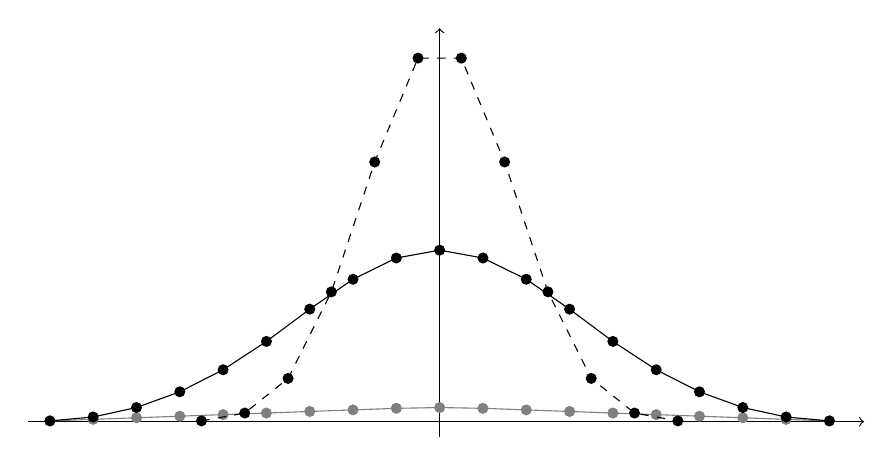
\begin{tikzpicture}[x=0.55cm,y=0.01cm]
  % Axes
  \draw[->] (-0.5,0) -- (18.8,0);
  %node[below] {$k$};
  \draw[->] (9,-20) -- (9,500);
  %node[left] {value};

  % x-axis ticks
  \foreach \k in {0,1,...,18} {
    %\draw (\k,0) -- (\k,-12);
    %node[below] {\scriptsize \k};
  }

    % ---- bottom row (gray) ----
  \foreach \k/\v in {
    0/1,1/3,2/5,3/7,4/9,5/11,6/13,7/15,8/17,9/18,10/17,11/15,12/13,13/11,14/9,15/7,16/5,17/3,18/1
  }{
    \fill[gray] (\k,\v) circle (2pt);
  }

    \draw[gray]
    (0,1)--(1,3)--(2,5)--(3,7)--(4,9)--(5,11)--(6,13)--(7,15)--(8,17)--(9,18)--
    (10,17)--(11,15)--(12,13)--(13,11)--(14,9)--(15,7)--(16,5)--(17,3)--(18,1);

  % ---- top rectangle distribution (black) ----
  \foreach \k/\v in {
    0/1,1/6,2/18,3/38,4/66,5/102,6/143,7/181,8/208,9/218,
    10/208,11/181,12/143,13/102,14/66,15/38,16/18,17/6,18/1
  }{
    \fill (\k,\v) circle (2pt);
  }

  \draw
    (0,1)--(1,6)--(2,18)--(3,38)--(4,66)--(5,102)--(6,143)--(7,181)--(8,208)--(9,218)--
    (10,208)--(11,181)--(12,143)--(13,102)--(14,66)--(15,38)--(16,18)--(17,6)--(18,1);

  % ---- Pascal row 11, symmetry-aligned ----
  % values: 1,11,55,165,330,462,462,330,165,55,11,1

   % Data points
  \foreach \k/\v in {3.5/1,4.5/11,5.5/55,6.5/165,7.5/330,8.5/462,9.5/462,10.5/330,11.5/165,12.5/55,13.5/11,14.5/1} {
    \fill (\k,\v) circle (2pt);
  }
  
  \foreach \k/\v in {
    3.5/1,4.5/11,5.5/55,6.5/165,7.5/330,8.5/462,
    9.5/462,10.5/330,11.5/165,12.5/55,13.5/11,14.5/1
  }{
    %\fill[red] (\k,\v) rectangle ++(0.28,0.28);
  }

  \draw[black,dashed]
    (3.5,1)--(4.5,11)--(5.5,55)--(6.5,165)--(7.5,330)--(8.5,462)--
    (9.5,462)--(10.5,330)--(11.5,165)--(12.5,55)--(13.5,11)--(14.5,1);
\end{tikzpicture}   
    \caption{Three significant rows in the intermediate configuration}
    \label{fig:threerows}
\end{figure}

If we look at the representation of the stable configuration in Figure~\ref{fig:stableconfign=9}, we see that the top of the middle part is more chaotic, while it gets more and more structured in the lower rows. The bottom triangle is very structured, so that we can even completely describe it through minimal rows. Not surprisingly, this description correlates with Figure~\ref{fig:threerows}, where the top plot, bell curve, is associated with randomness, and the bottom plot, arithmetic progression, is associated with structure.

We want to understand this change of structure better, so we look at the difference tables in the next section.








\section{Difference Tables}\label{sec:DiffTables}

We now define the table of differences between consecutive entries in $F(x, y)$. We define the \emph{difference table} $F'$ as follows:
\[F'(x,y) = F(x-1,y) - F(x,y-1).\]
\begin{example}
    For example,
    \[F'(1,0) = F(0,0) - F(1,-1) = 2^n\]
    and
    \[F'(0,1) = F(-1,0) - F(0,0) = -2^n.\]
\end{example}

\begin{example}\label{ex:Beginning_of_table}
Consider the top of the table $F(n)$ for $n>3$ as depicted in Figure~\ref{fig:Table1}. Then, we can compute the top of the corresponding difference table $F'(n)$, as depicted in Figure~\ref{fig:Table2}.
\begin{figure}[ht!]
\begin{center}
  \begin{tabular}{ccccccccc}
        & & &  & $2^n$  & & &  \\
      &  & & $2^{n-1}$ &  &  $2^{n-1}$ & &  \\  
      & & $2^{n-2}$ &  & $2^{n-1}$ & &  $2^{n-2}$ & \\ 
      & $2^{n-3}$ & & $3 \cdot 2^{n-3}$ & & $3 \cdot 2^{n-3}$ & & $2^{n-3}$ \\ 
      \textbf{$2^{n-4}$} & & $4 \cdot 2^{n-4}$ & & $6 \cdot 2^{n-4}$ & & $4 \cdot 2^{n-4}$  &  & \textbf{$2^{n-4}$} \\ 
  \end{tabular} 
\end{center}
  \caption{Top of the table $F(n)$ for $n > 3$ (only nonzero values).}
\label{fig:Table1}
\end{figure}
\begin{figure}[ht!]
\begin{center}
  \begin{tabular}{ccccccccccc}
      & & & & $2^n$ & & $-2^n$  & & & & \\
      & & & $2^{n-1}$ & & 0 & & $-2^{n-1}$ & & & \\  
      & & $2^{n-2}$ & & $2^{n-2}$ & & $-2^{n-2}$ & & $-2^{n-2}$ & &\\ 
      & $2^{n-3}$ & & $2 \cdot 2^{n-3}$ & & 0 & & $-2 \cdot 2^{n-3}$ & & $-2^{n-3}$ & \\ 
      $2^{n-4}$ & & $3 \cdot 2^{n-4}$ & & $2 \cdot 2^{n-4}$ & & $2 \cdot -2^{n-4}$ & & $-3 \cdot 2^{n-4}$  &  & $-2^{n-4}$. \\ 
  \end{tabular}
\end{center}
\caption{Top of the table $F'(n)$ for $n > 3$ (only nonzero values).}
      \label{fig:Table2}
\end{figure}
\end{example}

We see that the maximum absolute values in rows of $F'$, as we can see from Figure~\ref{fig:Table2} are
\[2^n,\ 2^{n-1},\ 2^{n-2},\ 2^{n-2},\ 3\cdot 2^{n-4}.\]
We see that this maximum sequence is weakly decreasing, and we will prove that later. We will also prove that in the left half of the difference table, the values weakly increase, then weakly decrease.

When we compute the difference tables $F'(n)$ for some large $n$, we notice consecutive entries that have the same value. Towards the bottom rows, we observe that these regions look like triangles. We illustrate this phenomenon for the table $F'(9)$ in Figure~\ref{fig:testingn9}. As before, we ignore zero values outside of the main shape and put the table horizontally to better fit the page.
\begin{figure}[h]
    \centering
    \includegraphics[width=1\linewidth]{DifferenceTableBoldDotsRegions.pdf}
    \caption{Consecutive regions, denoted by black dots, of $F'(9)$ where entries have the same value.}
    \label{fig:testingn9}
\end{figure}

We now prove general properties of difference tables. The first is analogous to Proposition~\ref{prop:symmetry}. The symmetry of the intermediate configuration implies the symmetry of the corresponding difference table.
\begin{proposition}[Symmetry]\label{prop:DiffTableSym}
    For each $i \geq 1$ and $j$, the $j$th leftmost element in row $i$ of $F'(n)$ is the same up to a sign as the $j$th rightmost element in that row: $F'(x,y) = -F'(y,x)$.
\end{proposition}

It is not surprising that the maximum element in rows of the intermediate configuration is not increasing. The next proposition shows that the same is true for difference tables, explaining that the rows of the intermediate configuration are becoming flatter. Due to symmetry, the maximum absolute value in a row of the difference table is the same as the maximum value on the left side of the row.

\begin{proposition}\label{prop:nonincreasingmax}
Let $n > 2$ and let $i> 1$. The maximum element of the $(i+1)$st row of $F'(n)$ is no greater than that of row $i$ of $F'(n)$.
\end{proposition}

\begin{proof}
We want to show that 
\[F'(x,y) \leq \max\{F'(x-1,y),F'(x,y-1)\}.\]
Due to symmetry, it is enough to look at the left side of the row. Suppose $a \le b \le c$ are three consecutive elements in row $i$ of $F$, which are all on the left side. Then the corresponding row in $F'$ has two consecutive elements $b-a$ and $c-b$.
    
The next row in $F$ has two consecutive elements $\floor{\frac{a}{2}} + \floor{\frac{b}{2}}$ and $\floor{\frac{b}{2}} + \floor{\frac{c}{2}}$. The next row in $F'$ has an element $\floor{\frac{c}{2}} - \floor{\frac{a}{2}}$. We need to show that
    \[\floor{\frac{c}{2}} - \floor{\frac{a}{2}} \le \max\{b-a,c-b\}.\]
    We have
    \[\floor{\frac{c}{2}} - \floor{\frac{a}{2}} \le \frac{c}{2} - \frac{a}{2} + \frac{1}{2}.\]
    Suppose $b-a \ne c-b$, then $\max\{b-a,c-b\} \ge \frac{c-a}{2} + \frac{1}{2}$. If $b-a = c-b$, then $a$ and $c$ have the same parity, and $\floor{\frac{c}{2}} - \floor{\frac{a}{2}} = \frac{c}{2} - \frac{a}{2} = b-a = c-b$. The statement follows. By symmetry, we get the statement when $a \ge b \ge c$.
    
    The only case that is left is when $a < b > c$. This only happens when $b$ is the central element, implying that $a = c$. In this case, 
    \[\floor{\frac{c}{2}} - \floor{\frac{a}{2}} = 0 \le \max\{b-a,c-b\},\]
    finishing the proof.
\end{proof}

% If we do not have floors, then we have a case similar to the distribution of entropy. Suppose we start with a row a, b, c. The differences are $(b-a) (c-b)$. The next row is (a+b)/2, (b+c)/2, with the difference (a-c)/2. Thus, the difference is the average of the previous differences and can't go up.

Each line of the table of intermediate configuration $F$ behaves similarly to a Gaussian probability density function $f(x) = \frac{1}{\sqrt{2\pi}}e^{-\frac{x^2}{2}}$. Like the Gaussian function for $x < 0$, the entry of $F$ increases as we move rightwards towards the center. In the left half of each row of the difference table $F'(n)$, the entries first weakly increase and then weakly decrease. The behavior of the row of $F'$ is similar to the behavior of the derivative of the Gaussian $f'(x) = -\frac{x}{\sqrt{2\pi}}e^{-\frac{x^2}{2}}$.

\begin{example}
Figure~\ref{fig:threerows_diffs} shows the differences for $n=11$ for the same rows as Figure~\ref{fig:threerows}. The differences for the last row of the top triangle (dashed line) are:
\[1,\ 10,\ 44,\ 110,\ 165,\ 132,\ 0,\ -132,\ -165,\ -110,\ -44,\ -10,\ -1;\]
The differences for the first row of the longest length in the intermediate configuration (black line) are:
\[1,\ 5,\ 12,\ 20,\ 28,\ 36,\ 41,\ 38,\ 27,\ 10,\ -10,\ -27,\ -38,\ -41,\ -36,\ -28,\ -20,\ -12,\ -5,\ -1;\]
the differences for the last row of the middle rectangle and the start of the bottom rectangle (gray line) are:
\[1,\ 2,\ 2,\ 2,\ 2,\ 2,\ 2,\ 2,\ 2,\ 1,\ -1,\ -2,\ -2,\ -2,\ -2,\ -2,\ -2,\ -2,\ -2,\ -1.\]
    \begin{figure}[ht!]
\centering
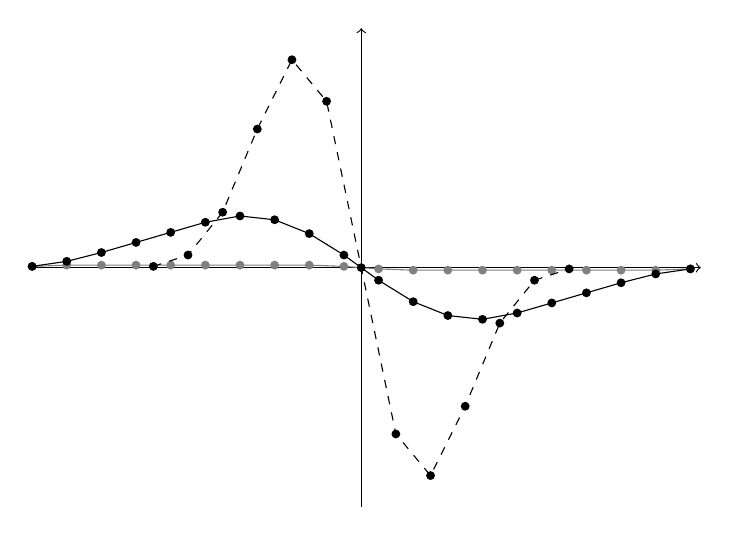
\begin{tikzpicture}[scale=0.8,x=0.55cm,y=0.02cm]
  % Axes (now centered to show positive/negative differences)
  \draw[->] (-0.5,0) -- (18.8,0);
  \draw[->] (9,-190) -- (9,190);

  % x-axis ticks (same as before)
  %\foreach \k in {0,1,...,18} {
  %  \draw (\k,0) -- (\k,-8);
  %}

  % ---- Gray (bottom row) first differences ----
  % original: 1,3,5,7,9,11,13,15,17,18,17,15,13,11,9,7,5,3,1
  % diffs:    2,2,2,2,2,2,2,2,1,-1,-2,-2,-2,-2,-2,-2,-2,-2
  \foreach \x/\v in {
    -0.5/1,0.5/2,1.5/2,2.5/2,3.5/2,4.5/2,5.5/2,6.5/2,7.5/2,8.5/1,9.5/-1,10.5/-2,11.5/-2,12.5/-2,13.5/-2,14.5/-2,15.5/-2,16.5/-2,17.5/-2,18.5/-1
  }{
    \fill[gray] (\x,\v) circle (2pt);
  }
  \draw[gray]
    (-0.5,1)--(0.5,2)--(1.5,2)--(2.5,2)--(3.5,2)--(4.5,2)--(5.5,2)--(6.5,2)--(7.5,2)--(8.5,1)--
    (9.5,-1)--(10.5,-2)--(11.5,-2)--(12.5,-2)--(13.5,-2)--(14.5,-2)--(15.5,-2)--(16.5,-2)--(17.5,-2)--(18.5,-1);

  % ---- Black (top rectangle distribution) first differences ----
  % original: 1,6,18,38,66,102,143,181,208,218,208,181,143,102,66,38,18,6,1
  % diffs:    5,12,20,28,36,41,38,27,10,-10,-27,-38,-41,-36,-28,-20,-12,-5
  \foreach \x/\v in {
    -0.5/1,0.5/5,1.5/12,2.5/20,3.5/28,4.5/36,5.5/41,6.5/38,7.5/27,8.5/10,9.5/-10,10.5/-27,11.5/-38,12.5/-41,13.5/-36,14.5/-28,15.5/-20,16.5/-12,17.5/-5,18.5/-1
  }{
    \fill (\x,\v) circle (2pt);
  }
  \draw
    (-0.5,1)--(0.5,5)--(1.5,12)--(2.5,20)--(3.5,28)--(4.5,36)--(5.5,41)--(6.5,38)--(7.5,27)--(8.5,10)--
    (9.5,-10)--(10.5,-27)--(11.5,-38)--(12.5,-41)--(13.5,-36)--(14.5,-28)--(15.5,-20)--(16.5,-12)--(17.5,-5)--(18.5,-1);

  % ---- Pascal row 11 (symmetry-aligned) first differences ----
  % x:      3.5,4.5,...,14.5
  % values: 1,11,55,165,330,462,462,330,165,55,11,1
  % diffs:  10,44,110,165,132,0,-132,-165,-110,-44,-10
  % midpoints x: 4.0,5.0,...,14.0
  \foreach \x/\v in {
  3.0/1,4.0/10,5.0/44,6.0/110,7.0/165,8.0/132,9.0/0,10.0/-132,11.0/-165,12.0/-110,13.0/-44,14.0/-10,15.0/-1
  }{
    {
    \fill (\x,\v) circle (2pt);
  }
  }
  \draw[black,dashed]
    (3.0,1)--(4.0,10)--(5.0,44)--(6.0,110)--(7.0,165)--(8.0,132)--(9.0,0)--(10.0,-132)--(11.0,-165)--(12.0,-110)--(13.0,-44)--(14.0,-10)--(15.0,-1);
\end{tikzpicture}
\caption{First differences of the three sequences in Figure~\ref{fig:threerows}.}
\label{fig:threerows_diffs}
\end{figure}
\end{example}

\begin{remark}
    One can observe that the entries do not necessarily first strictly increase and afterwards strictly decrease. To see this, consider the table of differences of consecutive entries in the difference table $F'(9)$, which we illustrate in Figure~\ref{fig:plusminustable} where bold black dots signify increases in entry, hollow dots signify two consecutive entries that are equal, and gray dots denote decreases in entries. This is analogous to viewing the sign of the second derivative of the probability density function $f$. The hollow dots in this figure correspond to two consecutive black dots in Figure~\ref{fig:testingn9}.
\end{remark}

\begin{figure}[ht!]
    \centering    \includegraphics[width=1.0\linewidth]{seconddiffs.pdf}
    \caption{Illustration of the sign of differences between entries in $F'(9)$. Bold black dots signify increases in entry in $F'(9)$, hollow dots signify two consecutive entries that are equal, and gray dots signify decreases in entries.}
    \label{fig:plusminustable}
\end{figure}

The following lemma shows that if three terms in the difference table weakly increase/decrease, then the two terms below also weakly increase/decrease.

\begin{lemma}\label{lem:IncreasingDiffTableSecondDeriv}
Suppose we have $F'(x_0, y_0+1) \leq F'(x_0-1, y_0+2) \leq F'(x_0-2, y_0+3)$, then $F'(x_0, y_0+2) \leq F'(x_0-1, y_0+3)$. Similarly, if $F'(x_0, y_0+1) \ge F'(x_0-1, y_0+2) \ge F'(x_0-2, y_0+3)$, then $F'(x_0, y_0+2) \ge F'(x_0-1, y_0+3)$.
\end{lemma}

\begin{proof}
To de-clutter the proof, let us denote $F(x_0,y_0)$ by $a$, $F'(x_0, y_0+1)$ by $d_1$, $F'(x_0-1, y_0+2)$ by $d_2$, and $F'(x_0-2, y_0+3)$ by $d_3$. We have $d_1 = F'(x_0, y_0+1) = F(x_0-1, y_0+1) - F(x_0,  y_0)$, $d_2 = F'(x_0-1, y_0+2) = F(x_0-2, y_0+2) - F(x_0-1, y_0+1)$, and $d_3 = F'(x_0-2, y_0+3) = F(x_0-3, y_0+3) - F(x_0-2, y_0+2)$. In the first part of the lemma, we are given that $d_1 \le d_2 \le d_3$.

We have
\[F(x_0-1, y_0+1) = a + d_1,\]
\[F(x_0-2, y_0+2) = a + d_1 + d_2,\]
\[F(x_0-3, y_0+3) = a + d_1 + d_2 + d_3.\]
Therefore,
\[F'(x_0, y_0+2) = \floor{\frac{a + d_1 + d_2}{2}} - \floor{\frac{a}{2}} \le \floor{\frac{a + 2d_2}{2}} - \floor{\frac{a}{2}} = d_2\]
and
\[F'(x_0-1, y_0+3) = \floor{\frac{a + d_1 + d_2 + d_3}{2}} - \floor{\frac{a+d_1}{2}} \ge \floor{\frac{a + d_1 + 2d_2}{2}} - \floor{\frac{a+d_1}{2}} = d_2.\]
The first part of the proposition follows. The second part follows by symmetry.
\end{proof}

\begin{theorem}
    In the left half of the difference table, the entries weakly increase and then weakly decrease.
\end{theorem}

\begin{proof}
We prove this via induction on row. 

For the base case, we look at row $0$ and directly observe that the statement is true for that row.

We can consider our rows to be infinite; we can assume that they start with zeros and end with zeros. Adding zeros at the beginning does not change the property that the row starts as weakly decreasing because nonzero terms at the beginning of the row are positive. For our inductive case, we suppose that the left half of row $i$ of the difference table first increases weakly, then decreases weakly. We observe that from Lemma~\ref{lem:IncreasingDiffTableSecondDeriv}, if we have three consecutive weakly increasing entries in the difference table, then, directly below, we have two consecutive weakly increasing entries in the next row.  Similarly, if we have three consecutive weakly decreasing entries in the difference table, then, directly below, we have two consecutive weakly decreasing entries in the next row. Using this fact and how the difference table first increases weakly and then decreases weakly in the left half of row $i$, we know that the same applies for row $i+1$.
\end{proof}



\section{Acknowledgments} 

The authors thank Professor Alexander Postnikov for suggesting the topic of chip-firing on posets, for helping formulate the project, and for helpful discussions. The MIT Department of Mathematics financially supports the first and second authors. The third author is supported by Harvard College.

All figures in this paper were generated using TikZ via \url{mathcha.io} and exported as PDF.
\bibliographystyle{unsrt}
\bibliography{biblio5.bib}

\smallskip

\noindent
Ryota Inagaki \\
\textsc{
Department of Mathematics, Massachusetts Institute of Technology\\
77 Massachusetts Avenue, Building 2, Cambridge, Massachusetts, U.S.A. 02139}\\
\textit{E-mail address: }\texttt{inaga270@mit.edu}
\medskip

\noindent
Tanya Khovanova \\
\textsc{
Department of Mathematics, Massachusetts Institute of Technology\\
77 Massachusetts Avenue, Building 2, Cambridge, MA, U.S.A. 02139}\\
\textit{E-mail address: }\texttt{tanyakh@yahoo.com}
\medskip

\noindent
Austin Luo \\
\textsc{
Harvard College,\\
1 Oxford Street,
Cambridge, MA 02138}\\
\textit{E-mail address: }\texttt{aluo@college.harvard.edu}
\medskip











\end{document}
